\documentclass[12pt]{article}
\usepackage[top= 3cm, bottom=2cm, left=2cm, right=2cm]{geometry}
\usepackage[utf8]{inputenc}
\usepackage{url}
\usepackage{hyperref}
\hypersetup{
    colorlinks=true,
    urlcolor=blue,
    linkcolor=blue,
    citecolor=blue
    }
\usepackage{graphicx}
\usepackage[sorting=none]{biblatex} %Imports biblatex package
\addbibresource{biblio.bib} %Import the bibliography file

\usepackage[breakable]{tcolorbox}
\usepackage{enumerate}
\usepackage[spanish]{babel}
\usepackage{csquotes}
\usepackage{todonotes}

%SIMBOLOS
\usepackage{amsfonts} 
\usepackage{amsmath}
\usepackage{MnSymbol}
\usepackage{wasysym}
\usepackage{marvosym}

\usepackage{amsthm}
\setlength {\marginparwidth }{2cm}

%LISTINGS%%%%%%%%%%%%%%%%%%%%%%%%%%%%%%%%%%
\usepackage{multirow}
\usepackage{xcolor}
\usepackage{listings}
\usepackage{comment}
\usepackage{courier}
%LISTING JAVA%%%%%%%%%%%%%%%%%%%%%%%%%%%%%%%%%%
\definecolor{dkgreen}{rgb}{0,0.6,0}
\definecolor{gray}{rgb}{0.5,0.5,0.5}
\definecolor{mauve}{rgb}{0.58,0,0.82}
\definecolor{gray97}{gray}{.97}

%usando lstdefinestyle {java}{otrasconf} se pueden usar varias diferentes, luego para usarlo \begin{lstlisting}[style=java]
\lstdefinestyle{java}{frame=Ltb,
    language=Java,
    framerule=0pt,
    rulesep=.4pt,
    backgroundcolor=\color{gray97},
    rulesepcolor=\color{black},
    aboveskip=3mm,
    belowskip=3mm,
    showstringspaces=false,
    columns=flexible,
    basicstyle=\small\ttfamily,
    numbers=left,
    numberstyle=\tiny\color{gray},
    keywordstyle=\color{blue},
    commentstyle=\color{dkgreen},
    stringstyle=\ttfamily\color{black},
    breaklines=true,
    breakatwhitespace=true,
    tabsize=3
}
\usepackage{caption}
\DeclareCaptionFormat{listing}{\rule{\dimexpr\textwidth+0pt\relax}{0.4pt}\par\vskip1pt#1#2#3}
\captionsetup[lstlisting]{format=listing,singlelinecheck=false, margin=0pt, font={sf},labelsep=space,labelfont=bf}

\renewcommand\lstlistingname{Código}

\DeclareMathVersion{sans}
\SetSymbolFont{operators}{sans}{OT1}{cmbr}{m}{n}
\SetSymbolFont{letters}  {sans}{OML}{cmbrm}{m}{it}
\SetSymbolFont{symbols}  {sans}{OMS}{cmbrs}{m}{n}

\lstnewenvironment{sflisting}[1][]
  {\lstset{#1}\mathversion{sans}}{}
%%%%%%%%%%%%%%%%%%%%%%%%%%%%%%%%%%%%%%%%%%%%
\usepackage{fancyhdr}
\pagestyle{fancy}

%%%COMPLETAR%%% 
\fancyhead[L]{Trabajo Práctico Obligatorio N°1 - Tecnologías Semánticas}
\fancyhead[R]{Agentes Inteligentes Para la Web}

\begin{document}
\begin{titlepage}
  \title{\textbf{Agentes Inteligentes Para la Web}\\
  %\vspace{2mm}
  \large{\textbf{Trabajo Práctico Obligatorio N°1 - Tecnologías Semánticas}}
  %\vspace{3mm}
  \author{
  Manuel Latorre FAI-1931\\ manuel.latorre@est.fi.uncoma.edu.ar\vspace{3mm}\\
  }}
  \date{Primer cuatrimestre 2023}

  \pagenumbering{gobble}
  \maketitle
  \vspace{25mm}
  \vfill
  \hspace*{-0.1in}{
  
\includegraphics[width=7cm, scale=0.5]{Images/Unco/faiLogo.png}
  \hspace*{1.5in}
  
\includegraphics[width=5cm, scale=0.5]{Images/Unco/Unco logo.png}
  }
\end{titlepage}

\titlepage

\newpage

\pagebreak

%INDICE Y FIGURAS
\newpage
\tableofcontents %%Indice
\listoffigures
\clearpage\pagenumbering{arabic}
\newpage

%INPUTS
\section{Ejercicio 1}
El dominio consistirá en la definición de diferentes tipos de animales junto con sus alimentos y habitats. De los animales se conocerá su nombre, tamaño promedio y peso promedio. De los alimentos se conoce su nombre y descripción. Del habitat en donde viven los animales se sabe el nombre, ubicación y clima. Los animales siempre serán o  terrestres o acuáticos, sin poder ser ambos a la vez. Ademas de los animales terrestres se pueden clasificar como cuadrúpedos o bípedos, mientras que los acuáticos se clasifican en cetáceos y peces. Finalmente de los animales acuáticos se conoce el tipo de agua en la que habitan, es decir dulce o salda
\begin{figure}[!h]
  \centering
  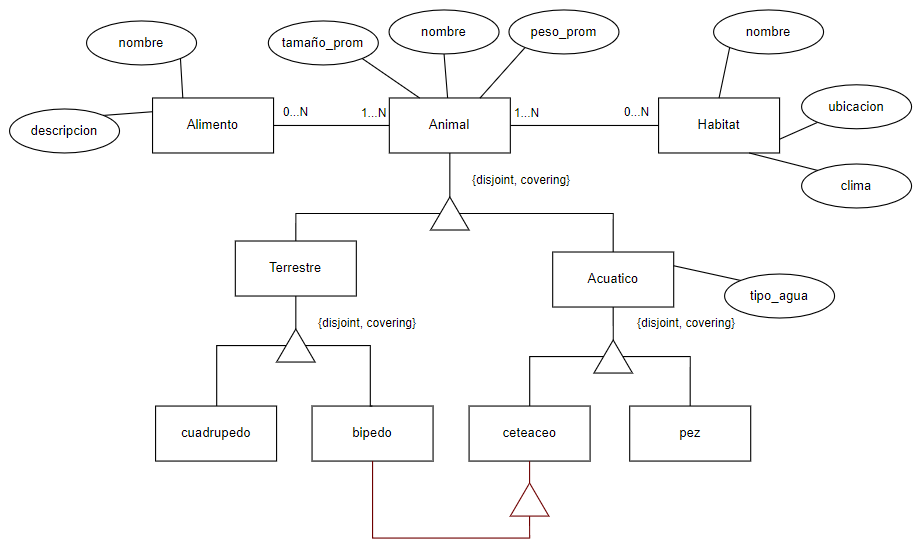
\includegraphics[width=16cm, scale=1]{Images/Imagenes/MER.png}
  \caption{Modelo entidad relación del dominio planteado junto con la inconsistencia}
  \label{fig:mer}
\end{figure}

En el MER planteado se puede observar en rojo una generalización especialización entre ``Cetaceo'' y ``Bipedo'', esta constituye una inconsistencia en el modelo debido a que las generalizaciones/especializaciones son totales y disjuntas por lo que si un ``Animal'' es ``Terrestre'' nunca podrá ser ``Acuático'' y al no poder ser ``Acuático'' entonces un ``Bipedo'' nunca debería poder ser un ``Cetaceo''. Esta relación se representa a traves de la lógica de la siguiente manera:
\begin{tcolorbox}
  Sea x un animal:
  
  \begin{center}
    $Cuadrupedo(x) \lor Bipedo(x) \longrightarrow Terrestre(x)$

    $Terreste(x) \longrightarrow \lnot Acuatico(x) $

    $Cuadrupedo(x) \longrightarrow \lnot Bipedo(x)$

    $Bipedo(x) \longrightarrow \lnot Cuadrupedo(x)$
    
    $Cetaceo(x) \lor Pez(x)\longrightarrow Acuatico(x)$

    $Acuatico(x) \longrightarrow \lnot Terrestre(x) $

    $Cetaceo(x) \longrightarrow \lnot Pez(x)$

    $Pez(x) \longrightarrow \lnot Cetaceo(x)$

    %$Terrestre(x) \land Cuadrupedo(x) \longrightarrow \lnot Bipedo(x) $
    %$Terrestre(x) \land Bipedo(x) \longrightarrow \lnot Cuadrupedo(x) $
  \end{center}
\end{tcolorbox}

Como se tiene que los ``Bipedos'' son animales ``Terrestres'' entonces se tiene que estos no pueden ser animales ``Acuaticos'' y por extension no pueden ser un ``cetaceos'', ya que si lo fueran también serian ``Acuaticos''. Por lo tanto queda claro que la especializacion/generalizacion entre ``Cetaceo'' y ``Bipedo'' no es posible dada la disyunción existente entre ``Terrestres'' y ``Acuaticos''. Por lo tanto, lo representado en rojo de la figura \ref{fig:mer} es efectivamente una inconsistencia en el modelo

\begin{tcolorbox}[title=Definicion con Lógicas Descriptivas]
\textbf{Habitat:}\\
$\exists clima \sqsubseteq Habitat$

$\exists nombre \sqsubseteq Habitat$

$\exists ubicacion \sqsubseteq Habitat$\\

\textbf{Alimento:}\\
$\exists nombre \sqsubseteq Alimento$

$\exists descripcion \sqsubseteq Alimento$\\

\textbf{Animal:}\\
$\exists nombre \sqsubseteq Animal$

$\exists peso\_prom \sqsubseteq Animal$

$\exists tamanio\_prom \sqsubseteq Animal$\\

\textbf{Terrestre:}\\
$Terrestre \sqsubseteq Animal \sqcap \lnot Acuatico$\\

\textbf{Acuatico:}\\
$Acuatico \sqsubseteq Animal \sqcap \lnot Terrestre$

$\exists tipo\_agua \sqsubseteq Acuatico$\\

\textbf{Cuadrupedo:}\\
$Cuadrupedo \sqsubseteq Terrestre \sqcap \lnot Bipedo$\\

\textbf{Bipedo:}\\
$Bipedo \sqsubseteq Terrestre \sqcap \lnot Cuadrupedo$\\

\textbf{Cetaceo:}\\
$Cetaceo \sqsubseteq Acuatico \sqcap \lnot Pez$\\

\textbf{Pez:}\\
$Pez \sqsubseteq Acuatico \sqcap \lnot Cetaceo$\\

\textbf{Relacion $\mathbf{Animal \leftrightarrow Habitat}$:}\\
$Animal \sqsubseteq \geq0 habita.Habitat$

$Habitat\sqsubseteq \exists esHabitado.Animal$\\

\textbf{Relacion $\mathbf{Animal \leftrightarrow Alimento}$:}\\
$Animal \sqsubseteq \geq0 come.Alimento$

$Alimento\sqsubseteq \exists esComido.Animal$
\end{tcolorbox}

\subsection{Validación con Protégé}
Al modelar la ontología en Protégé y validarla con el razonador HermiT, se puede detectar la presencia de inconsistencias. En la Figura 1, se muestra un ejemplo en el cual el razonador HermiT identifica una inconsistencia y proporciona una explicación para la misma.

La explicación del razonador indica que la clase ``Bipedo'' es una subclase de ``Cetaceo'', y a su vez, ``Cetaceo'' es una subclase de ``Acuatico''. Sin embargo, también se establece que ``Bipedo'' es una subclase de ``Terrestre'' y que ``Acuatico'' y ``Terrestre'' son clases disjuntas, lo que implica que no pueden tener instancias en común.

Esta explicación muestra que la existencia de ``Bipedo'' como subclase tanto de ``Cetaceo'' (que está relacionado con ``Acuatico'') como de ``Terrestre'' es contradictoria debido a la disyunción planteada entre ``Acuatico'' y ``Terrestre''. Por lo tanto, se demuestra la inconsistencia en el modelo ontológico y coincide con lo planteado a traves de la lógica previamente.

\begin{figure}[!h]
  \centering
  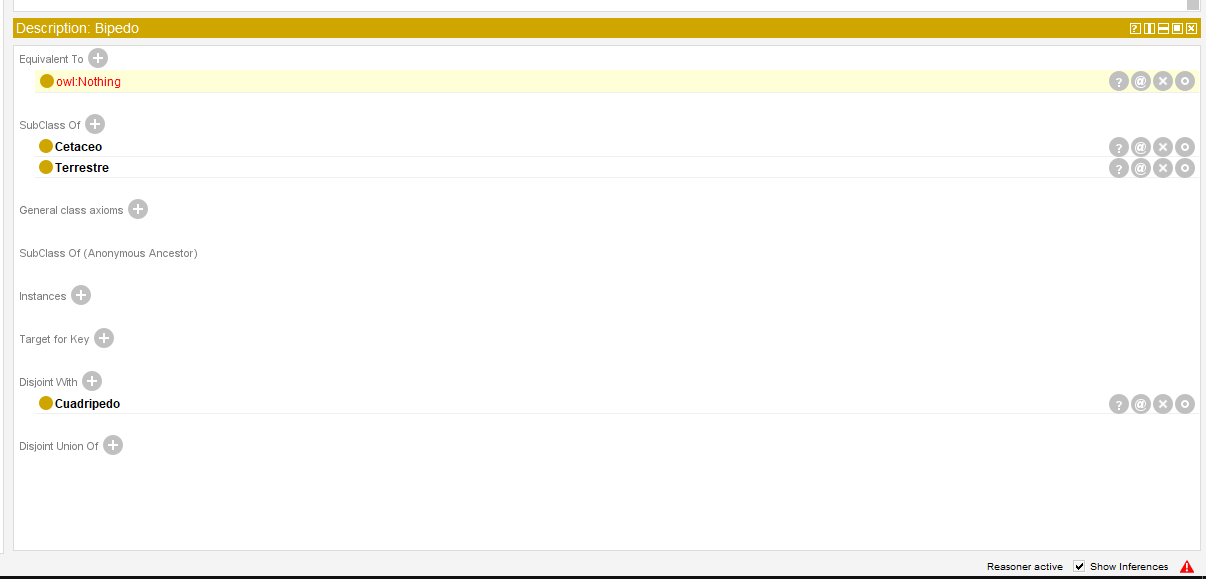
\includegraphics[width=16cm, scale=1]{Images/Imagenes/Protege1.png}
  \caption{Detección de inconsistencia en Bípedo}
  \label{fig:prot1}
\end{figure}

\begin{figure}[!h]
  \centering
  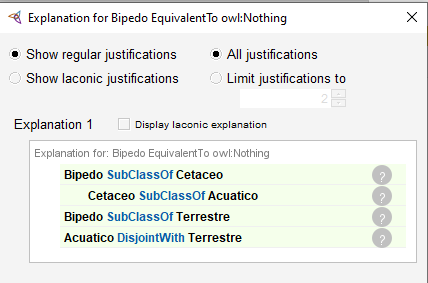
\includegraphics[width=10cm, scale=1]{Images/Imagenes/Protege2.png}
  \caption{Explicación del razonador HermiT a la inconsistencia encontrada en Bipedo}
  \label{fig:prot2}
\end{figure}

\subsection{Definición de relación en OWL y RDF}
Ademas de las diferencias sintácticas que se pueden apreciar entre las definiciones de Owl y RDF de los cuadros de mas abajo, aunque en el ejemplo planteado no se puede observar claramente, se debe destacar que OWL se basa en lógica descriptiva y permite expresar relaciones complejas y razonar sobre ellas. Ademas proporciona constructores específicos para definir jerarquías de clases, propiedades y restricciones que facilitan el razonamiento lógico.

En cambio RDF es un modelo de datos básico que se utiliza para la representación de la información
en la web semántica y no proporciona la capacidad de definir restricciones complejas o realizar razonamiento lógico directamente. RDF posee una expresividad mas limitada que OWL y se centra principalmente en la representación de tripletas sujetos-predicados-objetos sin proporcionar construcciones especificas para definir jerarquías o restricciones complejas
\begin{tcolorbox}[title=Definición en RDF de ``Acuatico'' subclase de ``Animal'' y disjunto con ``Terrestre'']
\begin{lstlisting}[language=XML, breaklines=true]
  <owl:Class rdf:about="http://tpo1#Animal">
      <rdfs:subClassOf rdf:resource="http://www.w3.org/2000/01/rdf-schema#Class"/>
  </owl:Class>
  
  <owl:Class rdf:about="http://tpo1#Acuatico">
      <rdfs:subClassOf rdf:resource="http://tpo1#Animal"/>
      <owl:disjointWith rdf:resource="http://tpo1#Terrestre"/>
  </owl:Class>
  
  <owl:Class rdf:about="http://tpo1#Terrestre">
      <rdfs:subClassOf rdf:resource="http://www.w3.org/2000/01/rdf-schema#Class"/>
  </owl:Class>
\end{lstlisting}
\end{tcolorbox}

\begin{tcolorbox}[title=Definición en RDF de ``Acuatico'' subclase de ``Animal'' y disjunto con ``Terrestre'']
  \begin{lstlisting}[language=XML, breaklines=true]
  <rdf:Description rdf:about="http://tpo1#Animal">
    <rdf:type rdf:resource="http://www.w3.org/2000/01/rdf-schema#Class"/>
  </rdf:Description>

  <rdf:Description rdf:about="http://tpo1#Acuatico">
    <rdf:type rdf:resource="http://www.w3.org/2000/01/rdf-schema#Class"/>
    <rdfs:subClassOf rdf:resource="http://tpo1#Animal"/>
    <rdfs:disjointWith rdf:resource="http://tpo1#Terrestre"/>
  </rdf:Description>

  <rdf:Description rdf:about="http://tpo1#Terrestre">
    <rdf:type rdf:resource="http://www.w3.org/2000/01/rdf-schema#Class"/>
  </rdf:Description>

  \end{lstlisting}
  \end{tcolorbox}


\section{Ejercicio 2}
\hypersetup{hidelinks}
\begin{tcolorbox}[title=Listar solo 10 propiedades del recurso Jorge Luis Borges \href{http://www.wikidata.org/entity/Q909}{\nolinkurl{http://www.wikidata.org/entity/Q909}}]

  \begin{lstlisting}[language=SPARQL, breaklines=true]
    PREFIX rdf: <http://www.w3.org/1999/02/22-rdf-syntax-ns#>
    PREFIX rdfs: <http://www.w3.org/2000/01/rdf-schema#>
    PREFIX owl: <http://www.w3.org/2002/07/owl#>
    PREFIX wd: <http://www.wikidata.org/entity/>
    
    SELECT ?property ?value
    WHERE {
      wd:Q909 ?property ?value.
      ?property rdf:type owl:ObjectProperty.
    }
    LIMIT 10
  \end{lstlisting}
  \end{tcolorbox}


\begin{tcolorbox}[title=Listar lugar de nacimiento y muerte. La consulta debe retornar también los rdfs:label filtrados por lenguaje inglés (usar FILTER)]

  \begin{lstlisting}[language=SPARQL, breaklines=true]
    PREFIX wdt: <http://www.wikidata.org/prop/direct/>
    PREFIX rdf: <http://www.w3.org/1999/02/22-rdf-syntax-ns#>
    PREFIX rdfs: <http://www.w3.org/2000/01/rdf-schema#>
    PREFIX owl: <http://www.w3.org/2002/07/owl#>
    PREFIX wd: <http://www.wikidata.org/entity/>

    SELECT *
    WHERE {
      wd:Q909 wdt:P19 ?bornPlace.  # Obtiene la propiedad "place of birth" de Q909
      wd:Q909 wdt:P20 ?deathPlace.  # Obtiene la propiedad "place of death" de Q909
      ?bornPlace rdfs:label ?bornPlaceLabel.  # Obtiene los labels de los valores
      ?deathPlace rdfs:label ?deathPlaceLabel.  # Obtiene el label del lugar de muerte
      FILTER(LANG(?bornPlaceLabel) = "en").
      FILTER(LANG(?deathPlaceLabel) = "en").
    }


  \end{lstlisting}
  \end{tcolorbox}

  \begin{tcolorbox}[title=Usando CONSTRUCT\, crear un nuevo grafo con todos los premios recibidos por Borges (award received). Recuperando también los rdfs:label de esos premios y filtrarlos por idioma inglés (en).]

    \begin{lstlisting}[language=SPARQL, breaklines=true]
      PREFIX wdt: <http://www.wikidata.org/prop/direct/>
      PREFIX rdf: <http://www.w3.org/1999/02/22-rdf-syntax-ns#>
      PREFIX rdfs: <http://www.w3.org/2000/01/rdf-schema#>
      PREFIX owl: <http://www.w3.org/2002/07/owl#>
      PREFIX wd: <http://www.wikidata.org/entity/>

      CONSTRUCT {
        wd:Q909 wdt:P166 ?award.
        ?award rdfs:label ?awardLabel.
      }
      WHERE {
        wd:Q909 wdt:P166 ?award. # Obtiene awards de q909
        ?award rdfs:label ?awardLabel. # Obteniene los labels de los awards
        FILTER(LANG(?awardLabel) = "en").
      }
  
  
    \end{lstlisting}
    \end{tcolorbox}

    \begin{figure}[!h]
      \centering
      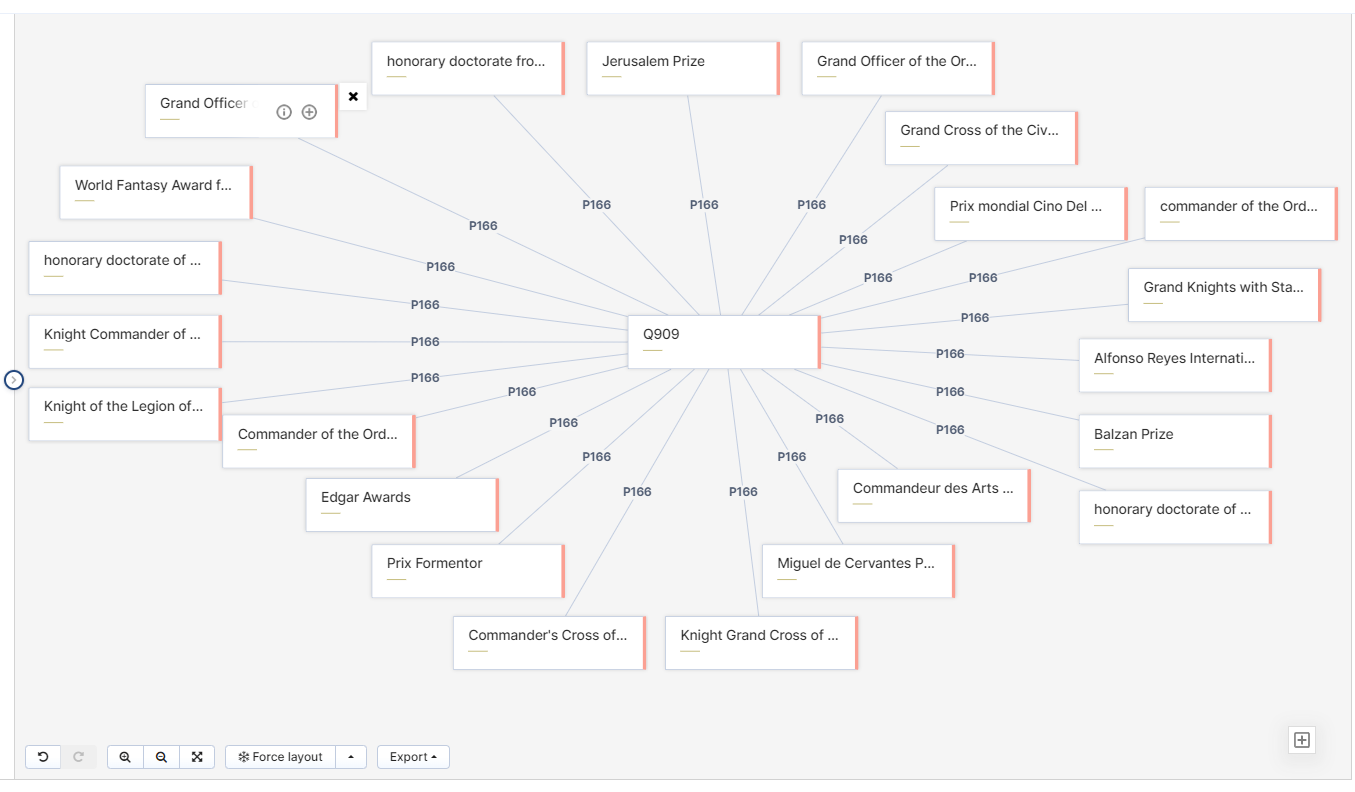
\includegraphics[width=16cm, scale=1]{Images/Imagenes/Grafo.png}
      \caption{Grafo de ``Awards'' de Borges obtenido con la ultima consulta SPARQL}
      \label{fig:marcado}
    \end{figure}
\section{Ejercicio 3}
Un agente deberia tener las siguientes cualidades para navegar la Web Semántica
\begin{itemize}
  \item El agente debe ser capaz de comprender cada declaración que recopila. Una forma de lograrlo es entendiendo los términos comunes y las relaciones que se utilizan para crear estas declaraciones, lo cual implica comprender los datos en formato RDF ya que proporcionan un modelo estandar para representar información semántica en la web, utilizando tripletas sujetos-predicados-objetos para expresar relaciones entre entidades. El agente debe ser capaz de interpretar dichas tripletas y completar la estructura y el significado de los datos RDF

  \item El agente debe ser capaz de realizar razonamientos basados en su comprensión de los términos y las relaciones comunes. Por ejemplo, al saber que los recursos A y B tienen la misma dirección de correo electrónico y considerar el conocimiento expresado por los términos y las relaciones comunes, debería ser capaz de concluir que A y B son en realidad el mismo recurso. Para esto se utilizan lógicas descriptivas ya que le dan la capacidad al agente de inferir nuevas conclusiones a partir de información disponible en las ontologías y los datos RDF. Estas lógicas proporcionan un marco formal para realizar inferencias y deducciones, lo que permite al agente obtener un mayor nivel de comprensión y conocimiento de los datos semánticos

  \item El agente debe ser capaz de procesar algunas consultas comunes que se realicen sobre las declaraciones que ha recopilado. Ya que, si no se proporciona una interfaz de consulta, las declaraciones recopiladas no serán de utilidad alguna. Aquí entra en juego SPARQL permitiéndole al agente ejecutar consultas sobre los datos RDF para obtener información especifica, brindándole la capacidad de buscar y filtrar datos según ciertos criterios.
  
  \item El agente debería ser capaz de utilizar ontologías para comprender la semántica de los datos y realizar razonamiento lógico sobre ellos. Las ontologías son modelos conceptuales que describen las relaciones y propiedades entre los diferentes elementos de un dominio de conocimiento, proporcionando una estructura formal para representar dicho conocimiento y permitiendo al agente inferir nuevas relaciones y conclusiones a partir de la información disponible.
\end{itemize}

\subsection{Web 2.0 vs Web Semantica}
Comparado con un agente para la Web 2.0, un agente para la Web Semántica tiene capacidades más avanzadas en términos de interpretación y comprensión del contenido. Mientras que un agente para la Web 2.0 generalmente se centra en la extracción de información basada en palabras clave y la búsqueda de contenido relevante, un agente para la Web Semántica puede entender la semántica subyacente de los datos y realizar inferencias lógicas sobre ellos. Esto permite al agente obtener un mayor nivel de conocimiento y comprensión, y proporciona la capacidad de realizar consultas más sofisticadas y contextualmente más relevantes. Además, un agente para la Web Semántica puede aprovechar la estructura y el significado de las ontologías para navegar y descubrir información de manera más precisa y eficiente, mientras que un agente para la Web 2.0 se basa principalmente en algoritmos de búsqueda de texto plano.

Un ejemplo claro donde se pueden ver las ventajas de la Web semantica sobre la Web 2.0 es en las implementaciones de ``mashups''. Un ``mashup'' es una aplicación web que recopila datos estructurados producidos por terceros a traves de APIs ofrecidas por dichos terceros, y procesa los datos de alguna manera para luego representarlos a los usuarios de una forma que difiere de su apariencia original. Normalmente, una aplicación de mashup mejora la presentación visual de los datos o ofrece un valor añadido a sus usuarios al combinar datos de diferentes fuentes, o ambas cosas. Este concepto esta mas relacionado con la Web 2.0, donde cada vez mas sitios web esconden su datos a traves de sus APIs. 

Un ``mashup'' implementado en Web 2.0 presenta la siguientes desventajas y complicaciones:

\begin{itemize}
  \item Limitada escalabilidad: La construcción de un ``mashup'' basado en APIs requiere aprender cada conjunto de APIs de diferentes proveedores, lo que implica un proceso constante de aprendizaje. Además, cada vez que haya un nuevo proveedor, será necesario aprender un nuevo conjunto de APIs. Por lo tanto, la construcción y mantenimiento de este tipo de ``mashup'' no es escalable y puede resultar costoso.
  \item Cobertura limitada: Un ``shopbot'' de una tienda digital, por ejemplo, solo puede comprender las APIs que se han programado para que entienda. No puede explorar por sí mismo, lo que limita la cobertura de datos. Cualquier decisión basada en este ``shopbot''probablemente no sea óptima debido a la limitada cobertura de datos.
  \item Desconexión con los proveedores de datos: Una vez que el ``shopbot'' recupera y consume los datos, se pierde el enlace entre este y el proveedor de datos original. Los usuarios no pueden regresar al sitio original que proporcionó los datos. Incluso si se incluyen enlaces que direccionan de vuelta a los proveedores de datos, estos enlaces suelen ser superficiales y no pueden llevar a ubicaciones precisas de los componentes de datos específicos. Esto limita la capacidad del usuario para aprovechar ofertas especiales u otras características ofrecidas en el sitio original.
\end{itemize}

En cambio con Web semantica a traves del uso de datos enlazados (\textit{Linked Data}) se obtendrán los siguientes resultados:
\begin{itemize}
  \item Buena escalabilidad del método en sí mismo: Bajo la Web de Datos Enlazados, los datos estructurados se expresan utilizando grafos y estándares RDF, que son un conjunto de estándares comunes a todos los sitios. Esto hace que la construcción y el mantenimiento de un mashup sean escalables, ya que no es necesario aprender constantemente nuevas APIs.
  \item Cobertura ilimitada de conjuntos de datos: A diferencia de los mashups de Web 2.0, las aplicaciones de Linked Data (Web semántica) operan sobre un espacio de datos global y sin límites. Esto les permite proporcionar respuestas más completas a medida que aparecen nuevas fuentes de datos en la Web.
  \item Enlaces cruciales para volver a los proveedores de datos: En los mashups de Linked Data, todos los elementos (recursos) se identifican mediante URIs controladas por el proveedor de datos. Si un usuario busca una de estas URIs, puede ser direccionado de vuelta al proveedor de datos original, quien puede proporcionar contenido adicional para dirigir el tráfico entrante. Esta capacidad de enlace es una diferencia clave entre los mashups de Web 2.0 y los mashups de Linked Data, y es donde reside el potencial valor comercial.
  \item Los mashups de Linked Data también ofrecen a los usuarios la posibilidad de enlazar casi ilimitadamente con otros recursos. Cada elemento en el mashup se identifica mediante una URI, que puede estar vinculada a otros recursos en otros conjuntos de datos. Estos enlaces también están tipificados, lo que permite al usuario seguirlos y visitar recursos específicos en otros conjuntos de datos. Esta capacidad de enlace ilimitado ofrece un valor significativo.
\end{itemize}

\printbibliography
\end{document}